%----------------------------------------------------

\begin{frame}
  \frametitle{Parallélisation de Routino}
  \begin{itemize}
  \item Séquentiel par portions
    \vspace{1em}
  \item Utilisation des données des précédentes portions
  \end{itemize}
\end{frame}

% --------------------------------------------------

\begin{frame}
  \frametitle{Parallélisation de Routino}

  \begin{itemize}
  \item Tour de France : en séquentiel
  \end{itemize}

  \begin{center}
    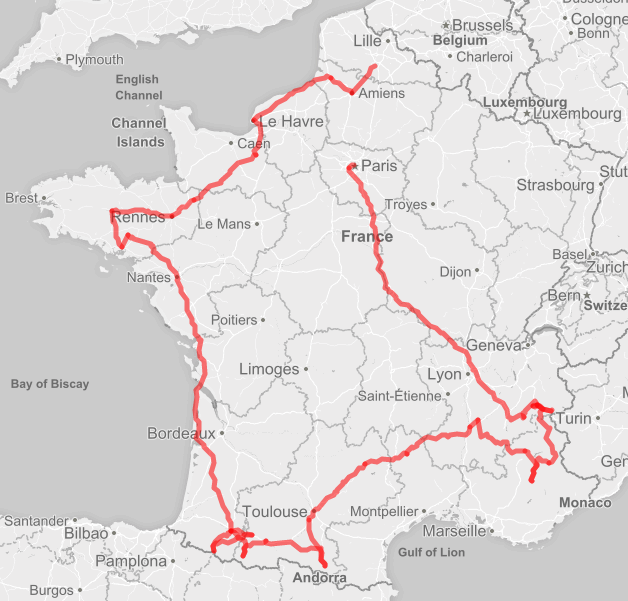
\includegraphics[scale=0.33]{include/tourfrance_mono.png}
  \end{center}

\end{frame}

% --------------------------------------------------

\begin{frame}
  \frametitle{Parallélisation de Routino}
  
  \begin{itemize}
  \item Tour de France : en parallèle
  \end{itemize}

  \begin{center}
    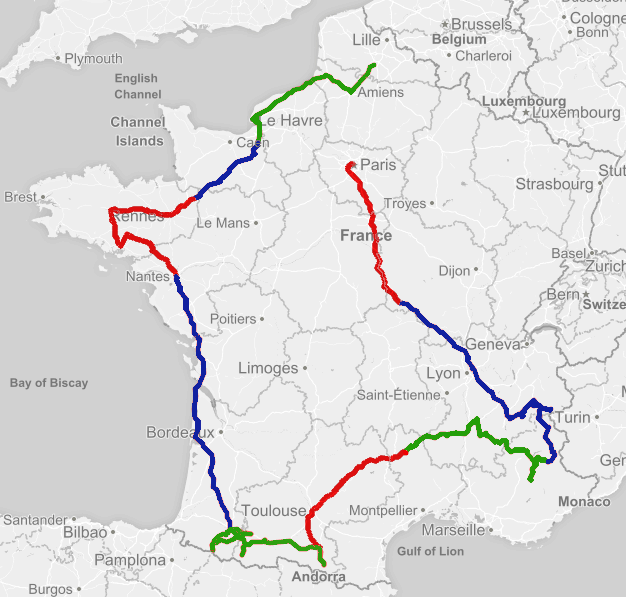
\includegraphics[scale=0.33]{include/tourfrance_multi.png}
  \end{center}
  
\end{frame}

% --------------------------------------------------

\begin{frame}
  \frametitle{Parallélisation de Routino}

  \begin{itemize}
  \item Rendre les portions indépendantes
    \vspace{1em}
  \item Minimiser les synchronisations
  \end{itemize}

\end{frame}

% --------------------------------------------------

\begin{frame}
  \frametitle{Parallélisation de Routino}

  \begin{center}
    \only<1>{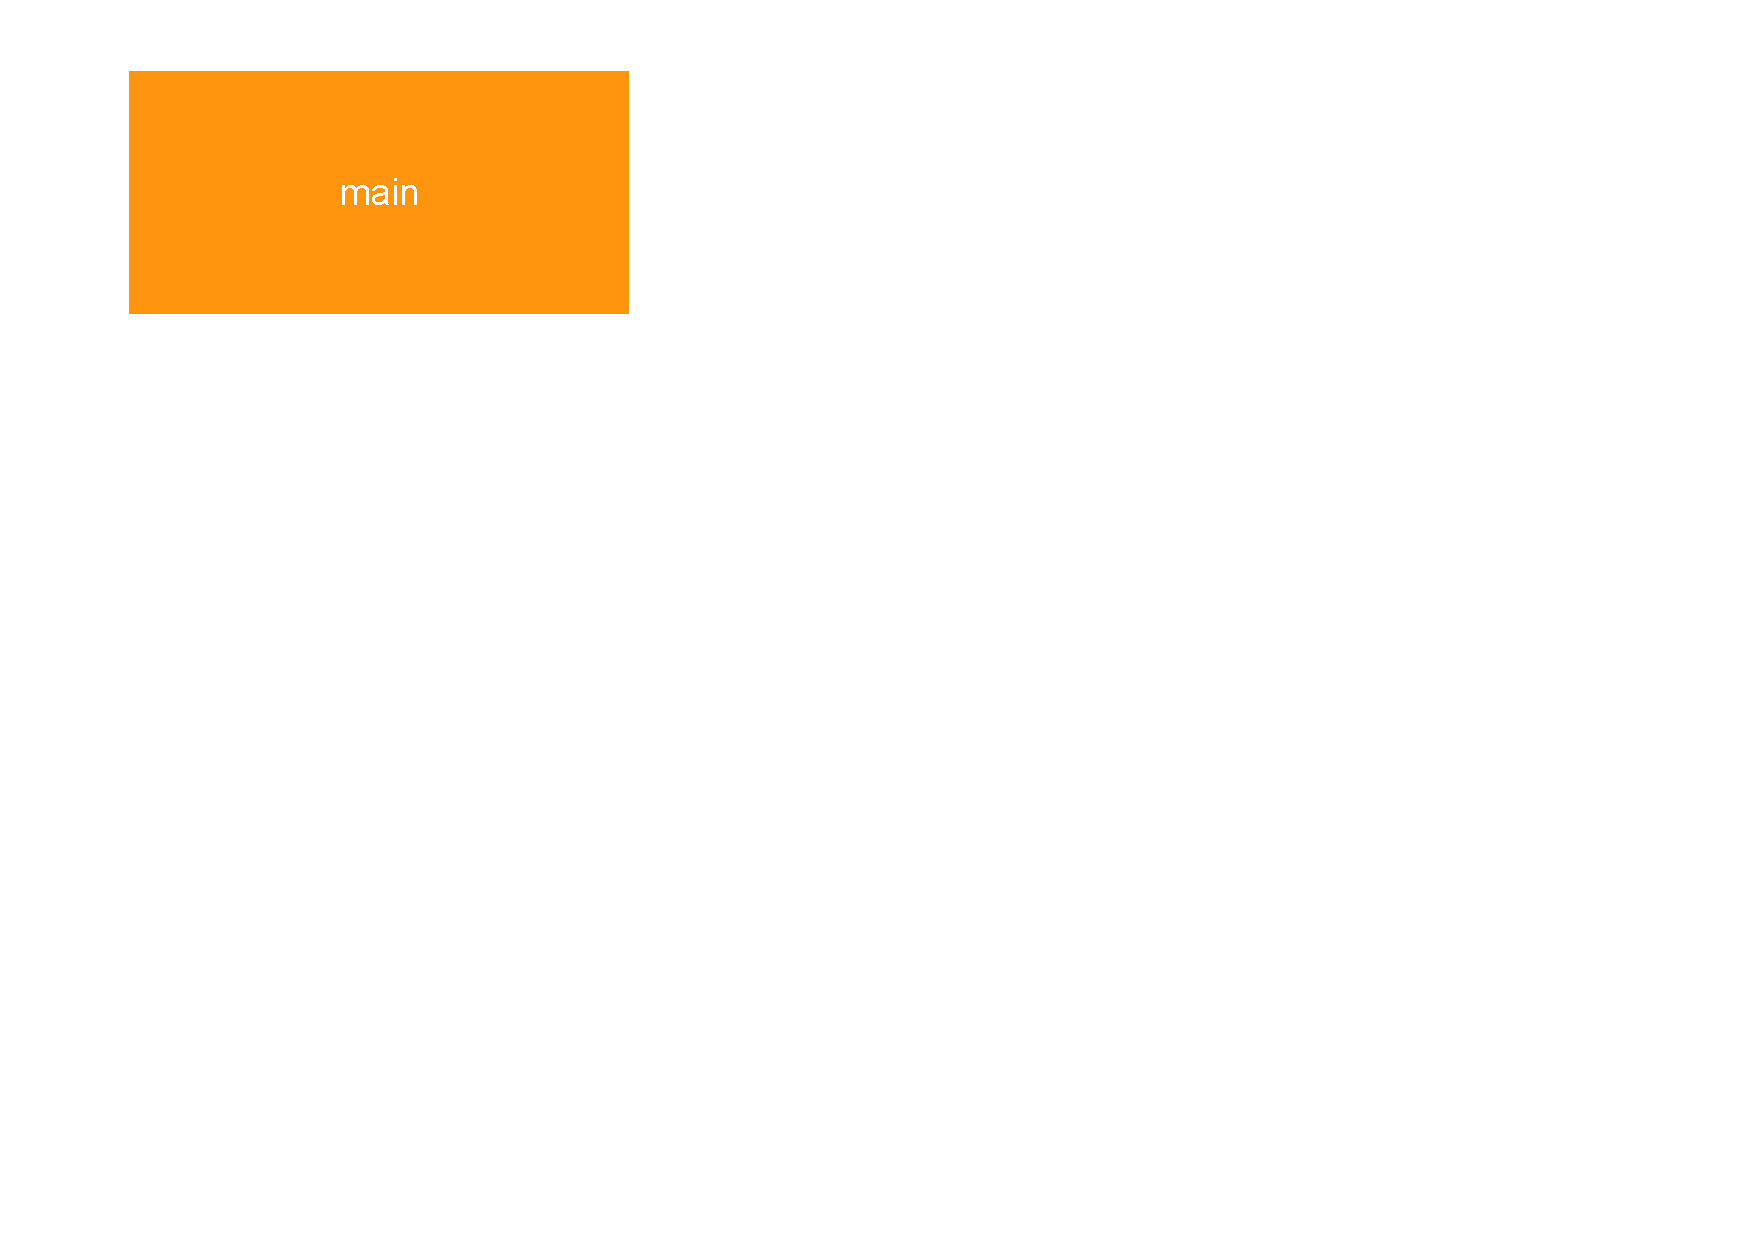
\includegraphics[scale=0.34]{include/multi1.pdf}}
    \only<2>{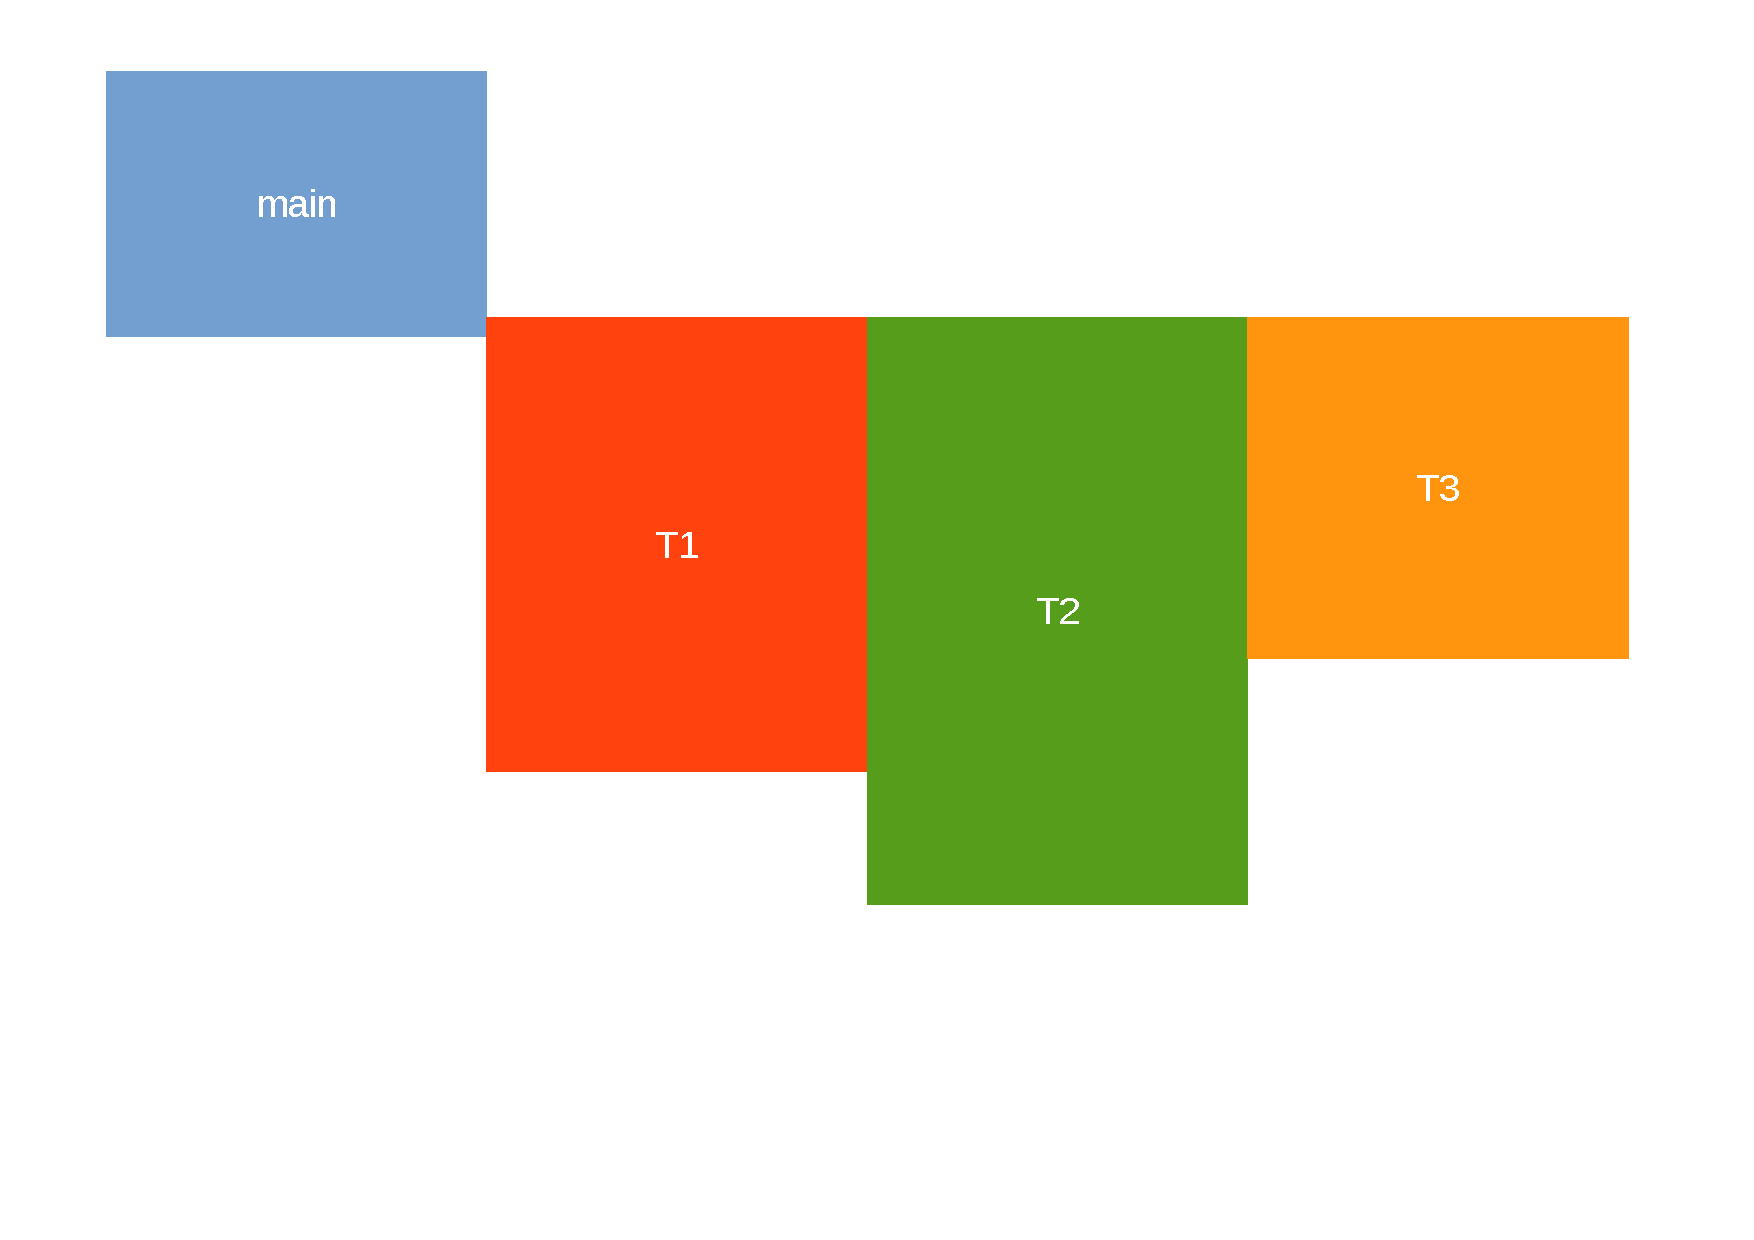
\includegraphics[scale=0.34]{include/multi2.pdf}}
    \only<3>{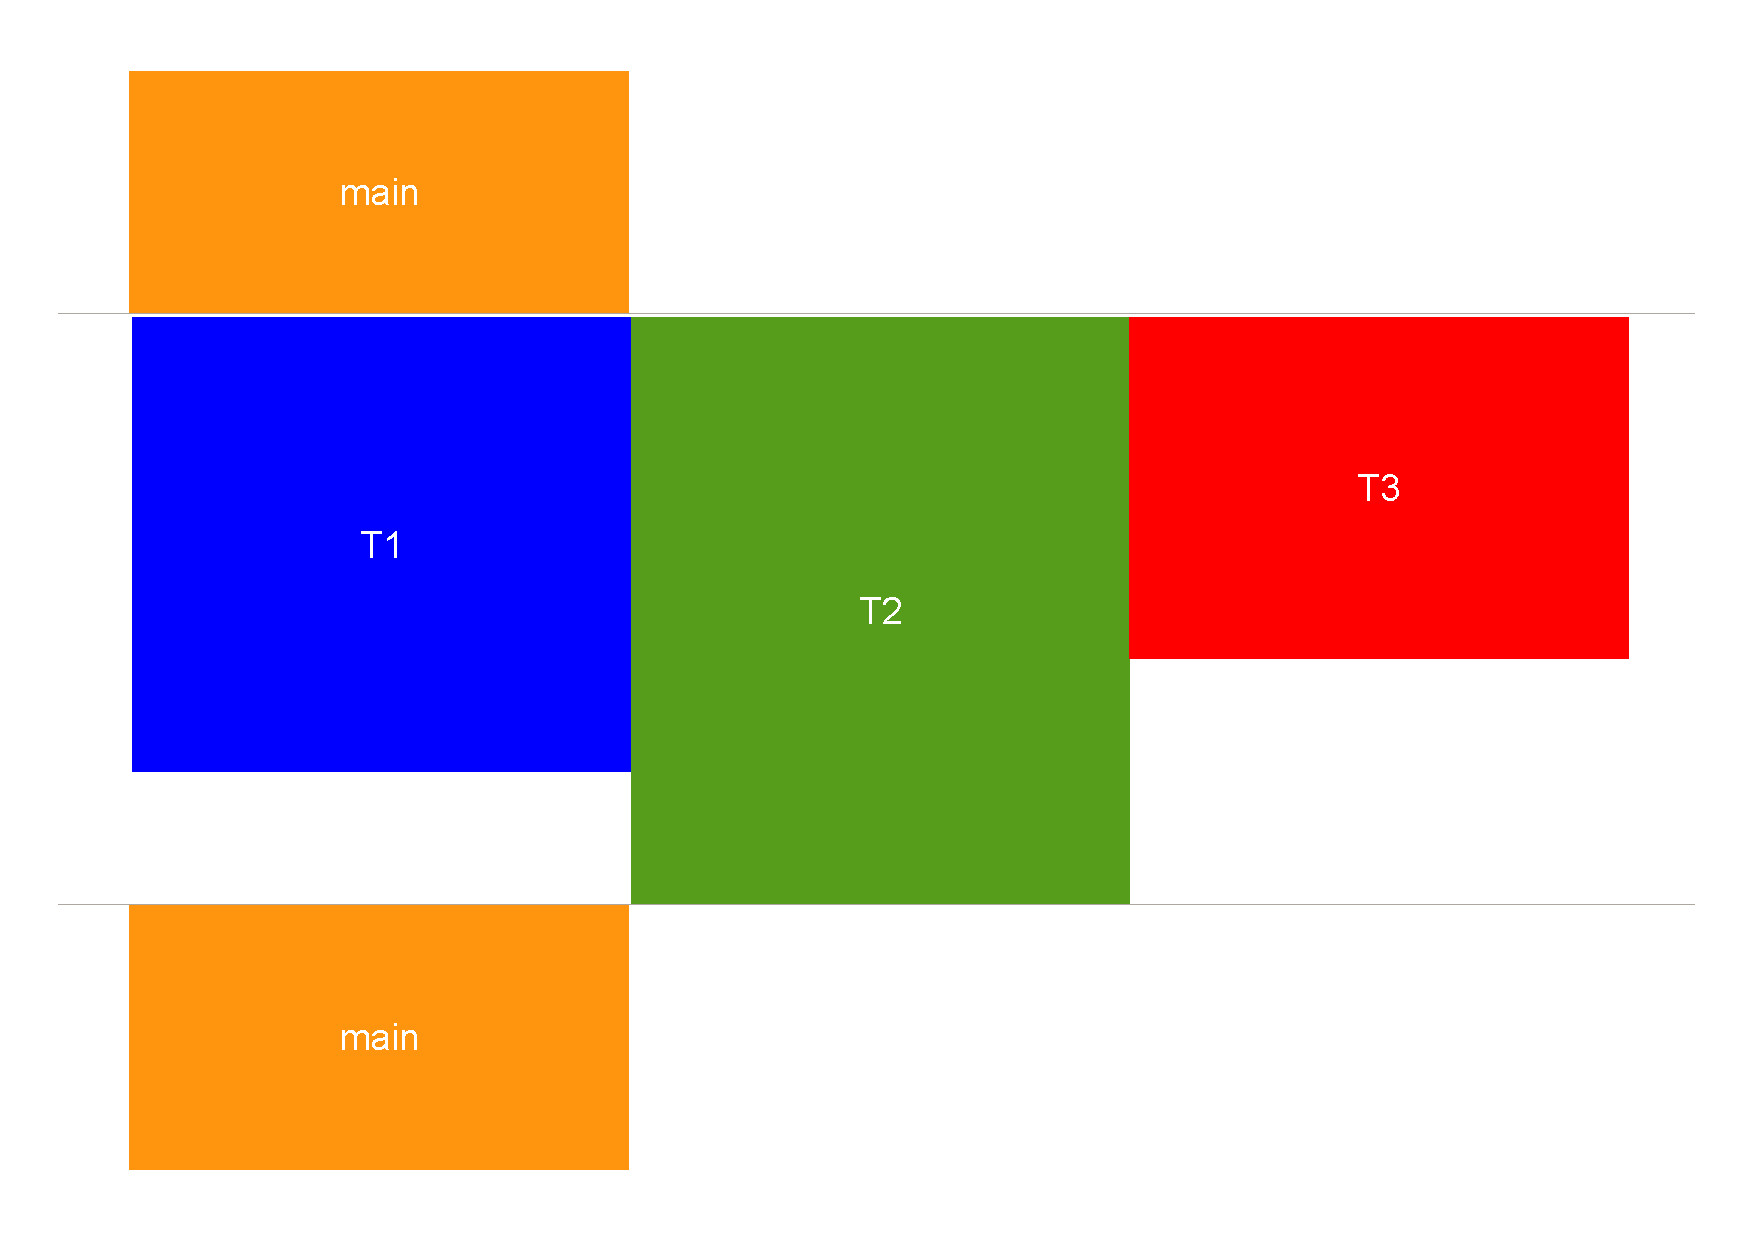
\includegraphics[scale=0.34]{include/multi3.pdf}}
  \end{center}

\end{frame}

% --------------------------------------------------

\begin{frame}
  \frametitle{\'Evaluation de la parallélisation}

  \only<1>{
    \begin{itemize}
    \item Utilisation CPU par coeur
    \end{itemize}
    
    \begin{center}
      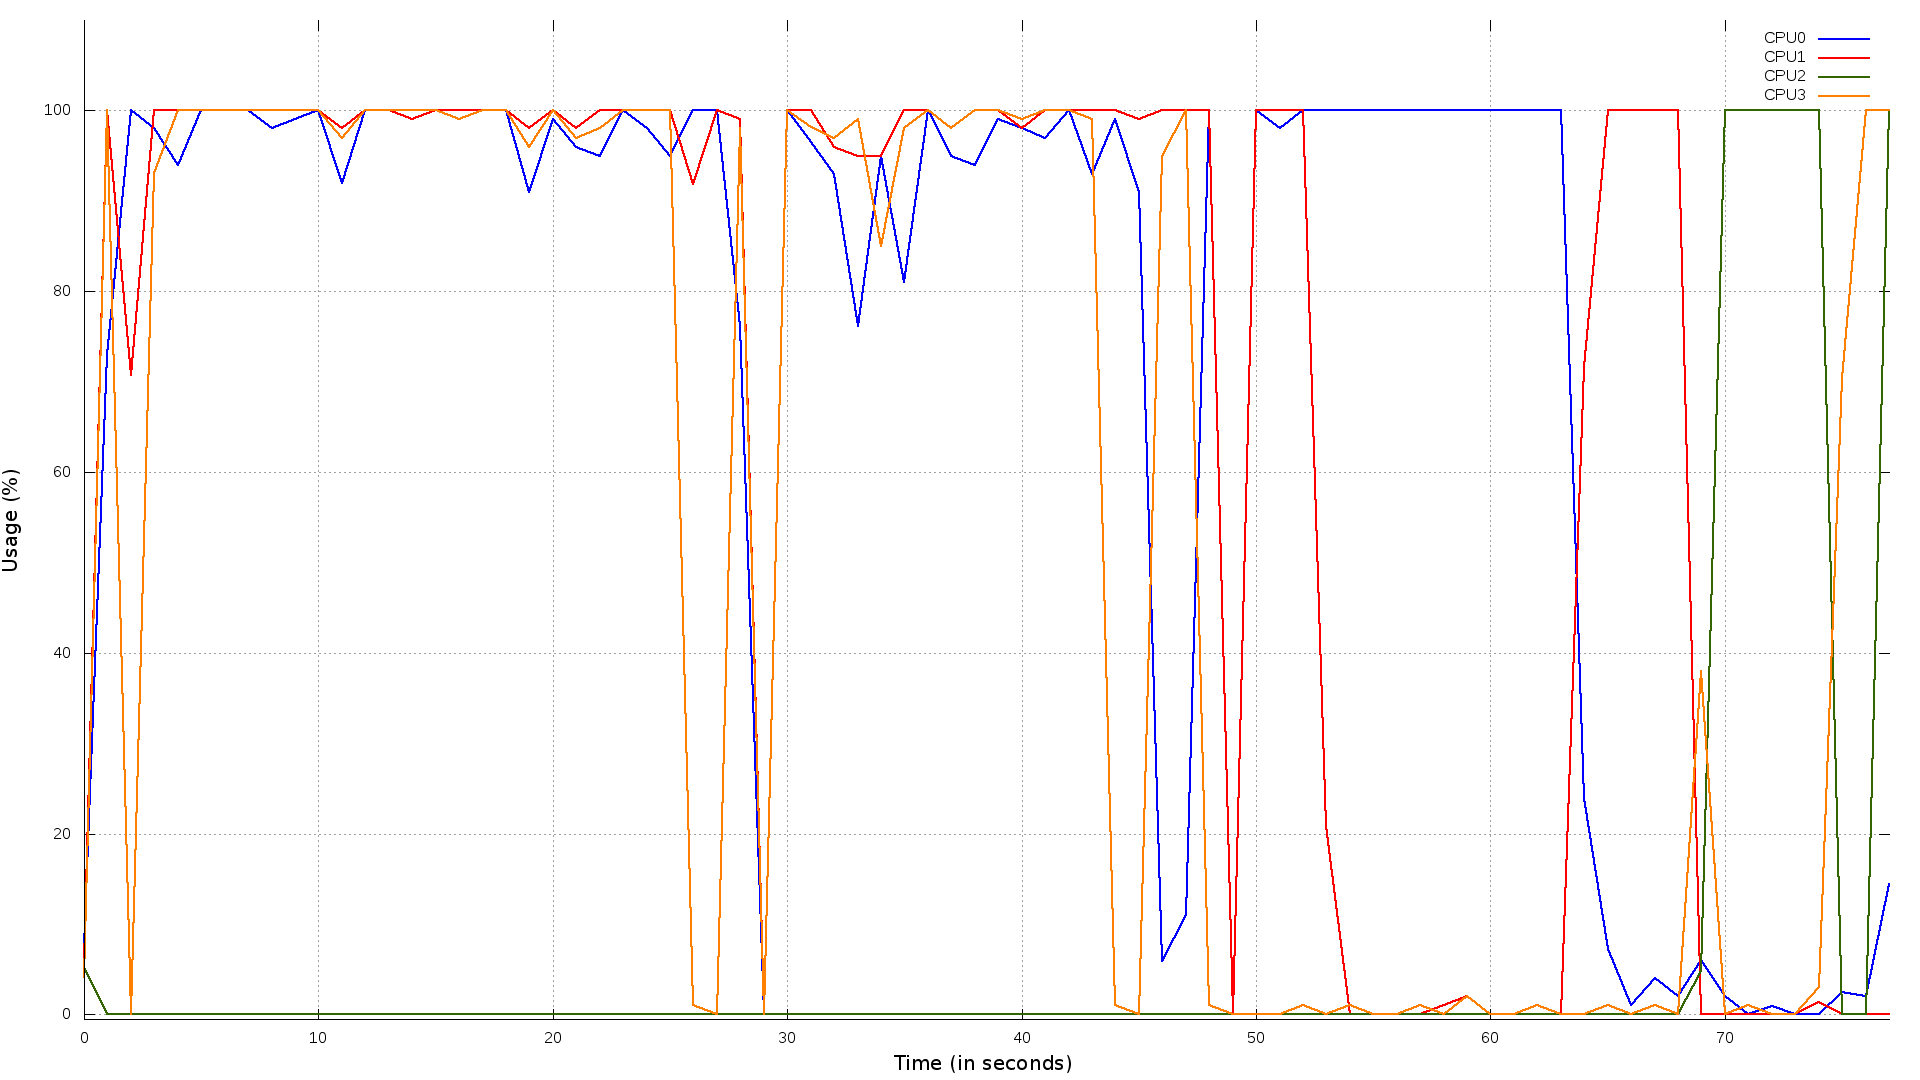
\includegraphics[scale=0.24]{include/cpu_usage.png}
    \end{center}
  }
  \only<2>{
    \begin{itemize}
    \item Utilisation CPU par tâche
    \end{itemize}
    
    \begin{center}
      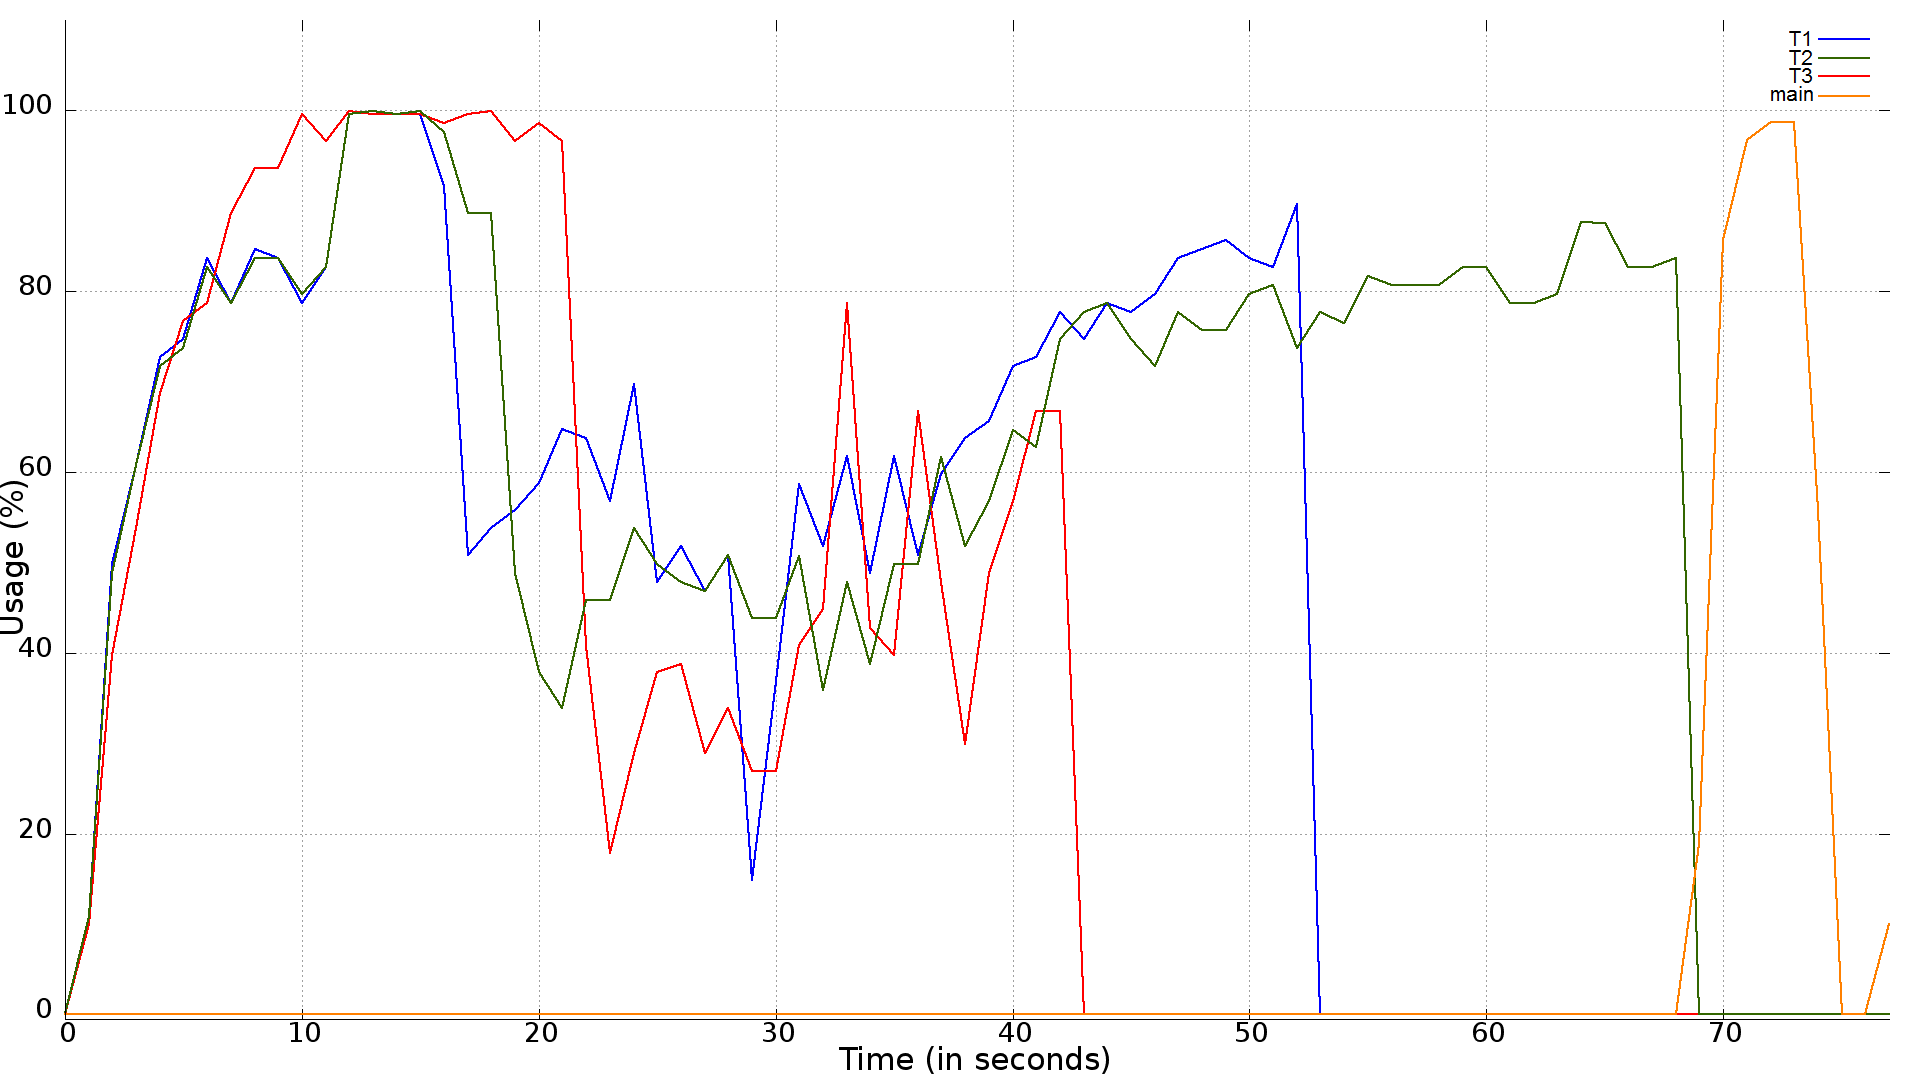
\includegraphics[scale=0.24]{include/thread_usage.png}
    \end{center}
  }
  
\end{frame}

% --------------------------------------------------
